%%%%%%%%%%%%%%%%%%%%%%%%%%%%%%%%%%%%%%%%%%%%%%%%%%%%%%%%%%%%%%%%%%%%%%%%%%%%%%%%
\chapter{Анализ исследований в области автоматического извлечения контрактов функций}
%%%%%%%%%%%%%%%%%%%%%%%%%%%%%%%%%%%%%%%%%%%%%%%%%%%%%%%%%%%%%%%%%%%%%%%%%%%%%%%%
В данном разделе проводится обзор контрактного программирования. Рассматривается использование контрактов в статическом анализе. Проводится обзор способов задания пользовательских спецификаций. Проводится анализ существующих в настоящий момент исследований в области автоматического извлечения контрактов.

%%%%%%%%%%%%%%%%%%%%%%%%%%%%%%%%%%%%%%%%%%%%%%%%%%%%%%%%%%%%%%%%%%%%%%%%%%%%%%%%
\section{Контрактное программирование}
%%%%%%%%%%%%%%%%%%%%%%%%%%%%%%%%%%%%%%%%%%%%%%%%%%%%%%%%%%%%%%%%%%%%%%%%%%%%%%%%
Контрактное программирование (design by contract, programming by contract, contract-based programming) --- это метод проектирования программного обеспечения. Он предполагает, что проектировщик должен определить формальные, точные и верифицируемые спецификации интерфейсов для компонентов системы. При этом, кроме обычного определения абстрактных типов данных, также используются <<контракты>> или утверждения(assertions).

Термин был введен Бертраном Мейером в связи с разработкой языка Eiffel и был описан в статье <<Design by contract>>\cite{designByContract} и книге <<Object-Oriented Software Construction>>\cite{oosc-meyer}. DbC появилось вследствие работ по формальной верификации, формальной спецификации и логики Хоара.

DbC является довольно простой, но, в то же время, мощной методикой, основанной на документировании прав и обязанностей программных модулей для обеспечения корректности программы. Основная идея контрактного программирования --- это модель взаимодействия элементов программной системы, основывающаяся на идее взаимных обязательств и преимуществ. Как и в бизнесе, <<клиент>> и <<поставщик>> действуют в соответствии с определенным контрактом. Контракты --- это булевы выражения, описывающие состояние программы. Выделяют три основных типа контрактов: предусловия, постусловия и инварианты.
\begin{itemize}
\item Предусловия --- обязательства, которые любой клиентский модуль должен выполнить перед вызовом вызовом метода. Если данные обязательства не выполнены, то метод не должен вызываться ни в коем случае. Эти предусловия дают преимущество поставщику --- он может не проверять выполнение этих предусловий;

\item Постусловия --- определенные свойства, которые выполняются после выполнения метода. Выполнение этих условий является обязательствами поставщика. Кроме того, наличие постусловий гарантирует завершение метода;

\item Инварианты --- свойства, которые должны выполняться и при вызове метода, и при выходе из него. Говоря об инвариантах обычно подразумевают инварианты класса --- глобальные свойства класса, определяющие более глубокие семантические свойства и ограничения целостности, характеризующие класс.
\end{itemize}

Многие языки программирования включают инструменты для задания подобных утверждений. Однако, DbC утверждает, что контракты являются ключевым инструментом создания корректного ПО, поэтому они должны быть утверждены на этапе проектирования. Таким образом, DbC предписывает начинать писать код с написания контрактов.

%%%%%%%%%%%%%%%%%%%%%%%%%%%%%%%%%%%%%%%%%%%%%%%%%%%%%%%%%%%%%%%%%%%%%%%%%%%%%%%%
\section{Контракты в статическом анализе}
%%%%%%%%%%%%%%%%%%%%%%%%%%%%%%%%%%%%%%%%%%%%%%%%%%%%%%%%%%%%%%%%%%%%%%%%%%%%%%%%
Статический анализ кода --- анализ программного обеспечения, производимый (в отличие от динамического анализа) без реального выполнения исследуемых программ. Статические методы анализа ПО очень часто кроме исходного кода так же используют дополнительные артефакты процесса компиляции: объектные файлы, промежуточные представления, спецификации, схемы алгоритмов. Статические методы анализа становятся все более популярными в наше время, так как развитие вычислительной техники позволяет снизить влияние одного из самых главных недостатков статических методов: высокой вычислительной сложности.

Статические методы можно разделить на методы верификации ПО и статический анализ ПО. Основным различием этих двух групп является то, что методы верификации основаны на применении математического аппарата для полного логического доказательства или опровержения каких-либо свойств кода, в то время как статический анализ представляет собой процесс аппроксимации кода, все доказываемые или опровергаемые им свойства носят вероятностный характер.

Главным достоинством верификации является ее математическая точность. Главным недостатком --- необходимость ручных подсказок о промежуточных и конечных целях доказательства и начальных условиях со стороны программиста. Эти условия, как правило, не могут быть построены ав­томатически и, подчас, требуют для своей формулировки не меньше усилий, чем сама программа.

К основным достоинствам статического анали­за относится то, что он может быть полностью автоматическим, осуществляет поиск ошибок без участия пользователя, и, соответствен­но, практически лишён влияния человеческого фактора. Кроме того, статический анализ ПО ориентирован, как правило, на поиск нефункциональных ошибок. К недостаткам данной группы подходов относят большие вычислительные затраты, наличие ложных обнаружений (в связи с аппроксимационной природой анализа), а также практически полное отсутствие возможности поиска функциональных ошибок.

Контрактное программирование как методика проектирования в современном мире используется достаточно редко. Исключениями являются только языки программирования, в которые DbC интегрирован изначально, и случаи, когда отсутствие ошибок в ПО является критическим. Основной причиной непопулярности DbC является необходимость ручного написания контрактов разработчиком. Зачастую это требует от него затрат большого количества времени и усилий. 

Однако, контракты часто применяются при статическом анализе и верификации как один из способов повышения полноты и точности. Для проведения анализа используют следующие критерии оценки корректности программных модулей:
\begin{itemize}
\item если инвариант класса и предусловия будут верны перед вызовом метода, то инвариант и постусловия будут верны после того, как метод завершит работу;

\item при вызове какого-либо метода программный модуль не должен нарушать его предусловия.
\end{itemize}

Существует множество инструментов статического анализа, поддерживающих контракты. Рассмотрим примеры подобных инструментов.

%%%%%%%%%%%%%%%%%%%%%%%%%%%%%%%%%%%%%%%%%%%%%%%%%%%%%%%%%%%%%%%%%%%%%%%%%%%%%%%%
\subsection{Библиотека CodeContracts}
%%%%%%%%%%%%%%%%%%%%%%%%%%%%%%%%%%%%%%%%%%%%%%%%%%%%%%%%%%%%%%%%%%%%%%%%%%%%%%%%
CodeContracts --- библиотека для платформы .NET от компании Microsoft, позволяющая задавать контракты в исходном коде\cite{codeContracts}. Библиотека позволяет работать с предусловиями, постусловиями и инвариантами. Пример приведен на листинге \ref{listing:codeContractsExample}. Для данной библиотеки так же разработано множество инструментов для автоматизации тестирования, автоматической генерации тестов, генерации документации, статического и динамического анализа.
\lstinputlisting[
label={listing:codeContractsExample},
caption={Пример задания контрактов с помощью библиотеки CodeContracts},
]{src/codeContractsExample.cs}

Одмин из таких инструментов является статический анализатор The Code Contracts static checker разработанный для библиотеки CodeContracts\cite{cccheck}. Статический анализ кода с помощью этого анализатора позволяет учитывать выполнение ранее заданных контрактов.

%%%%%%%%%%%%%%%%%%%%%%%%%%%%%%%%%%%%%%%%%%%%%%%%%%%%%%%%%%%%%%%%%%%%%%%%%%%%%%%%
\subsection{Статический анализатор Frama-C}
%%%%%%%%%%%%%%%%%%%%%%%%%%%%%%%%%%%%%%%%%%%%%%%%%%%%%%%%%%%%%%%%%%%%%%%%%%%%%%%%
Еще одним популярным инструментом является статический анализатор языка С Frama-C\cite{framaC}. Инструмент объединяет в себе несколько подходов к статическому анализу. В нем так же присутствует возможность задавать пользовательские спецификации на языке спецификаций ACSL\cite{acsl}. Этот язык позволяет задавать различные пользовательские спецификации, в том числе предусловия,постусловия и несколько видов инвариантов. Анализатор Frama-C затем проверяет выполнение заданных спецификаций.
\lstinputlisting[
label={listing:framaCExample},
caption={Пример задания спецификаций на языке ASCL},
]{src/framaCExample.c}

Стандартным способов задания контрактов для статических анализаторов (в том числе и для вышеописанных) является их ручное написание. При этом есть два разных способа, принципиально ничем не отличающихся: их описание на уровне исходного кода и задание с помощью какого-либо языка аннотаций. Минусы подобного подхода очевидны и полностью совпадают с минусами контрактного программирования: ручное написание контрактов требует большого количества усилий и времени.

%%%%%%%%%%%%%%%%%%%%%%%%%%%%%%%%%%%%%%%%%%%%%%%%%%%%%%%%%%%%%%%%%%%%%%%%%%%%%%%%
\section{Методы автоматического извлечения контрактов из исходного кода}
%%%%%%%%%%%%%%%%%%%%%%%%%%%%%%%%%%%%%%%%%%%%%%%%%%%%%%%%%%%%%%%%%%%%%%%%%%%%%%%%
Автоматическое и полуавтоматическое извлечение контрактов уже давно не является новой идеей. Оно начало развиваться уже в 2000х годах. При этом все исследования в этой области можно разделить на 
статический анализ исходного кода и документации и динамический подход, который основан на анализе выполнения программы.

Первые исследования в области автоматического извлечения контрактов проводились Николой Милановичем и Мирославом Малеком. Они опубликовали свои исследования в статье "Extracting Functional and Non-functional Contracts from Java Classes and Enterprice Java Beans"\cite{extractingContractsFromJava}. В этой работе они рассматривают способы извлечения предусловий, постусловий и инвариантов из исходного кода Java. Их идея основана на анализе методов класса, условий выбрасывания исключений и вызова методов, конструкторов класса и его базового класса, реализуемых интерфейсов. Так же в данной работе они рассматривают возможность извлечения контрактов из документации. Однако проблема в том что для этого необходим формальный инструмент анализа документации, создать который практически невозможно. Для извлечения контрактов они используют гибридный метод, основанный на комбинации динамического и статического анализа. Общая схема анализа, предлагаемого в их подходе приведена на рисунке \ref{image:milanovicExample}.
\begin{figure}[h!]
\center{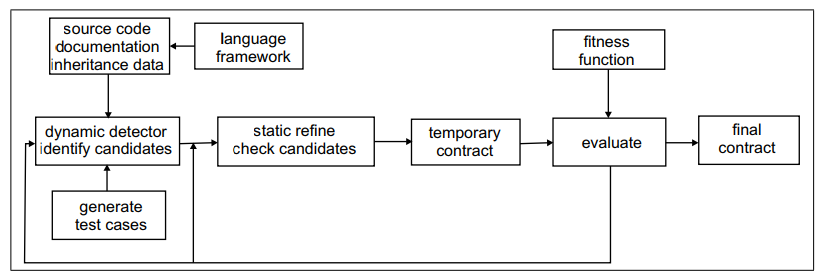
\includegraphics[width=\linewidth]{milanovicExample}}
\caption{Извлечение контрактов используя комбинацию статического и динамического анализа}
\label{image:milanovicExample}
\end{figure}

Параллельно с ними свои исследования проводили Бертранд Мейер и Карина Арнаут. В своей статье "Uncovering hidden contracts: the .NET example" они на примере анализа классов стандартной библиотеки .NET рассмотрели методологию извлечения контрактов\cite{uncoveringHiddenContracts}. В своей работе они основывались на статическом анализе метаданных компонентов .NET. Целью своей работы они ставят создание документированных оберток над стандартными классами .NET, а так же рассматривают способы расширения их методологии на другие языки. 

Автоматическое извлечение контрактов с помощью динамических методов впервые было рассмотрено в работах группы ученых из Университета Вашингтона: Майкла Эрнста, Джейка Кокрелла, Уильяма Грисуольда и Дэвида Ноткина. В 1999 году они опубликовали статью "Dynamically discovering likely program invariants to support program evolution", в которой они описали разработку инструмента Daikon\cite{discoveringInvariants}. Их подход основан на анализе трасс выполнения программы. Для получения данных трасс исполнения в их подходе используется автогенерация тестов несколькими способами. Данное исследование показало хорошие результаты и продолжило свое развитие. В настоящее время инструмент "The Daikon invariant detector" доступен для свободного пользования\cite{daikon}.

Примером более поздих работ в этой области является статья "Static specification inference using predicate mining"\cite{staticPredicateMining}. В этой работе рассматривается возможность автоматического извлечения спецификаций. При этом спецификации в ней делятся на два типа: контракты и спецификации библиотек. Спецификации извлекаются с помощью статических методов. Основная идея подхода: анализировать места вызова функций и пытаться выявлять шаблоны вызова функций. При этом шаблоны могут включать в себя различные проверки условий, вызовы других функций и т.д. Прототип, реализующий предложенную методику, был протестирован на большом количестве программ на языке С и показал неплохие результаты.

Одним из последних исследований в этой области является работа "Automatic extraction of assertions from execution traces of behavioural models"\cite{automiticAssertionsExtraction}. В данной работе описана разработка инструмента для автоматического извлечения темпоральных утверждений (temporal assertions) из трасс исполнения поведенческих моделей. Под темпоральными утверждениями при этом понимаются утверждения, являющиеся композицией обычных утверждений через темпоральные операторы. Разработанный инструмент использует гибридный подход: для изначального извлечения утверждений используется описанный ранее динамический инструмент Daikon, затем извлеченные утверждения сортируются, объединяются и выражаются через темпоральные операторы с помощью различных статических методов.

На основе проведенного обзора можно сделать вывод, что большинство современных подходов являются динамическими или гибридными. Это имеет свои недостатки, так как для использования динамических методов необходимо иметь возможность запуска программы и получения ее трасс выполнения. Это не всегда возможно. Существующие статические подходы можно расширить для получения более качественных результатов. Таким образом, разработка статического инструмента для автоматического извлечения контрактов из исходного кода является актуальной.

%%%%%%%%%%%%%%%%%%%%%%%%%%%%%%%%%%%%%%%%%%%%%%%%%%%%%%%%%%%%%%%%%%%%%%%%%%%%%%%%
\section{Резюме}
%%%%%%%%%%%%%%%%%%%%%%%%%%%%%%%%%%%%%%%%%%%%%%%%%%%%%%%%%%%%%%%%%%%%%%%%%%%%%%%%
В данном разделе проведен обзор контрактного программирования. Рассмотрены способы использования контрактов при статическом анализе. Проанализированы существующие подходы задания контрактов для исходного кода. Проведен обзор существующих исследований в области автоматического извлечения контрактов. На основе проведенного обзора обоснована актуальность разработки статического метода автоматического извлечения контрактов.